\documentclass[tikz,border=7pt]{standalone}
\usepackage[e]{esvect}
\usetikzlibrary{calc, angles}
\tikzset{
  line/.style = {
    shorten <=-3mm, shorten >=-3mm
  },
  vector/.style = {
    thick,-latex
  },
  dot/.style = {
    insert path={
      node[scale=2]{.}
    }
  },
  perp/.style = {
    draw,
    angle eccentricity=.5,
    angle radius=2mm,
    pic text=.
  }
}
\begin{document}
  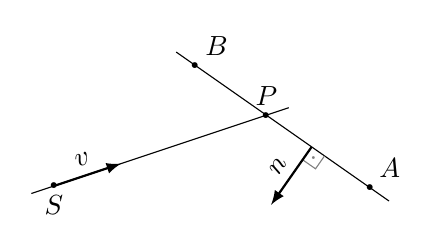
\begin{tikzpicture}[scale=0.9]
    % les coordonnées des points
    \path
      (0,0) coordinate (S)
      (3,1) coordinate (P)
      ($(S)!1cm!(P)$) coordinate (v)
      (2,1.7) coordinate (B)
      ($(B)!3cm!(P)$) coordinate (A)
      ($(B)!2cm!(P)$) coordinate (N)
      ($(N)!1cm!90:(B)$) coordinate (n)
    ;
    % les droites
    \draw
      (S) edge[line] (P)
      (A) edge[line] (B)
    ;
    % les vecteurs
    \draw
      pic[perp,gray]{right angle=n--N--A}
      (S) edge[vector] node[above, sloped]{$\vv{v}$} (v)
      (N) edge[vector] node[above, sloped]{$\vv{n}$} (n)
    ;
    % les points
    \path
      (S) [dot] node[below]{$S$}
      (P) [dot] node[above]{$P$}
      (A) [dot] node[above right]{$A$}
      (B) [dot] node[above right]{$B$}
    ;

  \end{tikzpicture}
\end{document}
